% =====================================================================
%  MẪU BÁO CÁO BÀI TẬP 1 — Giới thiệu ngành Trí tuệ Nhân tạo (CSC00006)
%  "Chân dung trợ lý AI"
% ---------------------------------------------------------------------
%  CÁCH DÙNG
%  1. Overleaf: New Project -> Upload Project -> chọn file zip này.
%     Menu -> Compiler: pdfLaTeX. Bấm Recompile.
%  2. Chọn hướng làm ở dòng \huongBtrue bên dưới (mặc định: Hướng A).
%  3. Thay mọi chỗ <...> bằng nội dung CỦA BẠN. Ảnh để trong images/.
%  4. Các nhãn [YC1]..[YC10] đánh dấu chỗ đáp ứng 10 yêu cầu kỹ thuật
%     ở mục 3 đề bài. Trước khi nộp, dò lại đủ 10 nhãn là yên tâm.
%  5. Khi xong, có thể xoá nhánh của hướng bạn KHÔNG làm cho gọn.
% =====================================================================
\documentclass[12pt,a4paper]{article}

% ---------- Tiếng Việt (pdfLaTeX) ----------
\usepackage[utf8]{inputenc}
\usepackage[T5]{fontenc}
\usepackage[vietnamese]{babel}

% ---------- Trình bày ----------
\usepackage[margin=2.5cm]{geometry}
\usepackage{amsmath,amssymb}
\usepackage{graphicx}          % \includegraphics
\usepackage{booktabs}          % \toprule \midrule \bottomrule
\usepackage{float}             % [H] = đặt hình/bảng đúng chỗ
\usepackage{pgfplots}          % vẽ biểu đồ (Hướng B)
\pgfplotsset{compat=1.18}
\usepackage{xurl}               % cho phép ngắt dòng URL dài tự nhiên
\usepackage[hidelinks]{hyperref} % \url, link bấm được trong PDF
\graphicspath{{images/}}

\begin{document}

% =====================================================================
% [YC1] TRANG BÌA
% =====================================================================
\begin{titlepage}
  \centering
  {\large TRƯỜNG ĐẠI HỌC KHOA HỌC TỰ NHIÊN -- ĐHQG-HCM\\
   KHOA CÔNG NGHỆ THÔNG TIN\par}
  \vspace{3.5cm}
  {\Large\bfseries BÁO CÁO BÀI TẬP 1\par}
  \vspace{0.3cm}
  {\large Môn: Giới thiệu ngành Trí tuệ Nhân tạo (CSC00006)\par}
  \vspace{1.2cm}
  {\huge\bfseries Chân dung trợ lý AI:\\ Google Gemini\par}
  \vfill
  \begin{tabular}{rl}
    Sinh viên: & <Họ và tên> \\
    MSSV:      & <MSSV> \\
    Lớp:       & <Lớp> \\
    Giảng viên:& Trần Huy Bân \\
  \end{tabular}
  \par\vspace{1.5cm}
  TP. Hồ Chí Minh, \today
\end{titlepage}

% =====================================================================
% [YC2] TÓM TẮT + MỤC LỤC TỰ ĐỘNG
% =====================================================================
\begin{abstract}
Bài viết này tìm hiểu về công cụ Gemini của Google thông qua các thông tin cơ bản như nguồn gốc, cách hoạt động, tính năng và các gói sử dụng. Đồng thời, bài viết cũng đưa ra những trải nghiệm thực tế của bản thân mình qua các ví dụ làm tốt và trả lời sai, từ đó phân tích những hạn chế về hiện tượng ảo giác và quyền riêng tư dữ liệu. Bên cạnh đó, bài báo cáo đối chiếu với các quy định hiện hành về liêm chính học thuật khi dùng AI trong giáo dục. Cuối cùng, mình đúc kết lại các kỹ năng cần thiết và đưa ra định hướng về cách sử dụng AI có trách nhiệm trong suốt 4 năm đại học.
\end{abstract}

\tableofcontents
\newpage

% =====================================================================
% [YC3] BÁO CÁO CHI TIẾT (HƯỚNG A: GOOGLE GEMINI)
% =====================================================================

% [YC3] Ít nhất 3 mục lớn (\section), có mục con (\subsection)
\section{Giới thiệu}
\subsection{Lý do chọn Gemini}
Gemini là mô hình trí tuệ nhân tạo xử lý đa phương thức, hỗ trợ công việc và học tập một cách hiệu quả, tích hợp sâu vào hệ sinh thái Google giúp thuận tiện cho công việc và trò chuyện theo thời gian thực.
Sự phù hợp của Google Gemini trong công việc và học tập xuất phát từ việc Gemini có khả năng hiểu và phản hồi các yêu cầu phức tạp, đa dạng, hỗ trợ nhiều ngôn ngữ và định dạng dữ liệu khác nhau, giúp người dùng dễ dàng tiếp cận và sử dụng. Đồng thời, giới hạn token không quá ít và tốc độ trả lời nhanh, đáp ứng tốt nhu cầu của đại đa số người dùng.
Bên cạnh đó, Google còn hỗ trợ sinh viên với việc miễn phí một năm gói Google AI Plus và giảm giá cho sinh viên ở các gói khác, giúp các bạn có thể dễ dàng tiếp cận công nghệ hơn.
Đặc biệt, mình chọn Gemini là vì mình am hiểu nhiều nhất về công cụ này nhờ việc đã trực tiếp sử dụng nó trong một thời gian dài.

\subsection{Sử dụng Gemini trong các tác vụ hằng ngày}
Hằng ngày, mình sử dụng Gemini (Chatbot) cho đa số mọi tác vụ như soạn lịch, hỏi đáp các thông tin thường ngày và sử dụng phiên bản Agent (Antigravity Agent) để xây dựng những phần mềm mình mong muốn nhằm phục vụ các nhu cầu cơ bản trong cuộc sống của mình.%
\footnote{Các thử nghiệm và khảo sát trong báo cáo được thực hiện trên phiên bản Gemini Web; cụ thể sử dụng Gemini Flash-Lite 3.5 cho việc hỏi câu hỏi đơn giản, Gemini Flash 3.8 cho tác vụ thông thường và Gemini 4 Argon cho các tác vụ phức tạp như code (thời điểm ghi nhận: tháng 10/2026).}

\section{Nguồn gốc}
Gemini (tiền thân là Google Bard) được phát triển bởi Google DeepMind và Google Research, đứng đầu bởi các chuyên gia AI hàng đầu thế giới. Bảng~\ref{tab:mocs} tóm tắt các cột mốc chính trong lịch sử phát triển của công cụ dựa trên thông tin tổng hợp từ Wikipedia~\cite{wiki-gemini} và các thông cáo công nghệ chính thức của Google.

\begin{table}[H]
  \centering
  \caption{Các cột mốc phát triển chính của Google Gemini}
  \label{tab:mocs}
  \begin{tabular}{lp{11.5cm}}
    \toprule
    Thời điểm & Sự kiện \\
    \midrule
    12/2023 & Ra mắt Gemini 1.0 với 3 phiên bản Nano, Pro, Ultra; với mô hình Gemini 1.0 Ultra đạt tới trình độ ngang với chuyên gia con người trên benchmark MMLU~\cite{team2023gemini}. \\
    02--05/2024 & Ra mắt Gemini 1.5 Pro với cửa sổ ngữ cảnh kỷ lục 1 triệu tokens~\cite{team2024gemini}~\cite{google-gemini-15-pro}; sau đó bổ sung phiên bản Gemini 1.5 Flash tối ưu tốc độ và chi phí tính toán~\cite{google-gemini-15-flash-debut}. \\
    11/2024 & Ra mắt Gemini 2.0 Flash, mở đầu kỷ nguyên Agent với khả năng tự thực thi tác vụ nhiều bước, hỗ trợ input/output đa phương tiện và tính năng Deep Research~\cite{google-gemini-2-agent}. \\
    02--03/2025 & Công bố Gemini 2.0 Pro, Gemini 2.0 Flash-Lite~\cite{google-gemini-2-updates-feb2025}; tiếp nối là Gemini 2.5 Pro với khả năng suy nghĩ (thinking process) trước khi trả lời~\cite{comanici2025gemini}~\cite{google-gemini-25-thinking-mar2025}. \\
    05--06/2025 & Mở rộng họ mô hình với Gemini 2.5 Flash, Gemini 2.5 Flash-Lite và ra mắt công cụ dòng lệnh mã nguồn mở Gemini CLI~\cite{google-gemini-cli}. \\
    11--12/2025 & Ra mắt Gemini 3 Pro với tư duy suy nghĩ sâu (Deep Think), đồng thời giới thiệu nền tảng tác tử tự hành Antigravity và phiên bản Gemini 3 Flash~\cite{google-gemini-3}. \\
    02--05/2026 & Ra mắt Gemini 3.1 Pro với năng lực xử lý chuyên sâu vượt trội; giới thiệu trợ lý chủ động Gemini Spark, mô hình đa phương thức sinh video Gemini Omni, Gemini 3.5 Flash và Antigravity 2.0~\cite{google-spark-omni}. \\
    07/2026 & Phát hành Gemini 3.6 Flash, Gemini 3.5 Flash-Lite và Gemini 3.5 Flash-Lite Cyber chuyên dụng cho an toàn thông tin~\cite{techcrunch-gemini-models-2026}. \\
    09--10/2026 & Ra mắt kiến trúc thế hệ mới Gemini 4 Argon, tăng cường tối đa năng lực lập trình và khả năng đối thoại kỹ thuật chuyên sâu~\cite{google-gemini-4-argon}. \\
    \bottomrule
  \end{tabular}
\end{table}

\section{Cách hoạt động ở mức khái niệm}
\subsection{Mô hình ngôn ngữ lớn là gì?}
Mô hình ngôn ngữ lớn (LLM) dùng cấu trúc mạng neuron (Transformer), hoạt động theo cách dự đoán xác suất từ tiếp theo sẽ xuất hiện chứ không hẳn là có khả năng hiểu như con người. Bằng việc nạp càng nhiều dữ liệu trong quá trình huấn luyện, mô hình có thể hoàn thiện mạng neuron và điều chỉnh các tham số phù hợp, giúp câu trả lời tự nhiên giống con người và dự đoán từ ngữ ngày càng tốt hơn.

Ví dụ về một số mô hình LLM phổ biến hiện nay:
\begin{itemize}
  \item GPT (OpenAI)
  \item LLaMA (Meta)
  \item Claude (Anthropic)
  \item Gemini (Google)
\end{itemize}

\subsection{Token là gì?}
Token là đơn vị cơ bản được sử dụng trong các mô hình AI. Thông thường, một token tương ứng với khoảng 4 ký tự trong tiếng Anh, hoặc khoảng 1.5 ký tự trong tiếng Việt có dấu. Tuy vậy, do AI không hiểu chữ viết trực tiếp nên các chữ sẽ được chuyển đổi toàn bộ thành các vector số (embedding) và đưa vào các tầng neuron để tính toán.

Khi sử dụng thực tế, người dùng thường quan tâm tới hai loại token:
\begin{enumerate}
  \item \textbf{Đầu vào / Ngữ cảnh (Context Window):} Số lượng token tối đa mà mô hình có thể ghi nhớ và xử lý cùng lúc để trả lời câu hỏi.
  \item \textbf{Đầu ra (Output Token):} Lượng token tối đa mà mô hình được phép sinh ra cho một câu trả lời duy nhất.
\end{enumerate}

Các loại token phổ biến trong hệ thống đa phương thức:
\begin{itemize}
  \item \textbf{Text and Symbol Tokens:} Dùng cho văn bản, mã nguồn (Code), ký tự đặc biệt, các thẻ cấu trúc prompt.
  \item \textbf{Vision Tokens:} Lưới ảnh tĩnh (Vision Transformer patches), các khung hình video theo chuỗi thời gian.
  \item \textbf{Audio Tokens:} Biểu đồ phổ Mel (Mel Spectrogram), mã nén âm thanh rời rạc.
\end{itemize}

\subsection{Đoán từ tiếp theo}
Mô hình tính xác suất của một câu $w_1, w_2, \dots, w_n$ bằng cách nhân xác suất của từng token khi biết các token đứng trước, xem~\eqref{eq:lm}:
\begin{equation}
  P(w_1,\dots,w_n) = \prod_{t=1}^{n} P(w_t \mid w_1,\dots,w_{t-1}).
  \label{eq:lm}
\end{equation}

Xác suất cho từng token tiếp theo thường tính bằng hàm softmax:
\begin{equation}
  P(w_t = i \mid \cdot) = \frac{e^{z_i}}{\sum_{j=1}^{|V|} e^{z_j}},
  \label{eq:softmax}
\end{equation}
trong đó $z_i$ là ``điểm'' mô hình gán cho token $i$ và $|V|$ là kích thước bộ từ vựng. Nền tảng của các mô hình này là kiến trúc Transformer~\cite{vaswani2017}.

\section{Tính năng và các gói sử dụng}
Gemini cho phép sử dụng rất nhiều tính năng hữu ích:
\begin{itemize}
  \item Xử lý đa phương thức: văn bản, hình ảnh, âm thanh, và nhiều định dạng file khác nhau.
  \item Khả năng suy luận logic và giải quyết vấn đề toán học.
  \item Hỗ trợ lập trình (Code), gỡ lỗi và giải thích thuật toán.
  \item Cửa sổ ngữ cảnh lớn: giúp người dùng có thể cung cấp nhiều dữ liệu đầu vào cùng một lúc.
  \item Tích hợp sâu vào hệ sinh thái Google: Google Calendar, Google Docs, Google Sheets, Google Drive.
  \item Giao diện sử dụng dễ dàng, trực quan với nhiều tính năng nâng cao.
  \item Tốc độ phản hồi nhanh.
  \item Gemini Spark có khả năng truy cập vào hệ sinh thái Google của bản thân để dễ dàng trả lời, có thể lập lịch và lập kế hoạch một cách tự động mà không phụ thuộc vào việc máy tính có đang mở hay không.
  \item Tính năng Agent (Antigravity) cho phép AI có thể chủ động ``làm'' thay vì chỉ có ``nói''.
\end{itemize}

\begin{table}[H]
  \centering
  \caption[So sánh gói miễn phí và trả phí của Gemini Web]{So sánh gói miễn phí và trả phí của Gemini Web (tra cứu ngày 15/10/2026)\footnotemark}
  \label{tab:goi}
  \begin{tabular}{llp{7.2cm}}
    \toprule
    Tiêu chí & Miễn phí (Free) & Trả phí (Google One AI Pro) \\
    \midrule
    Giá / tháng & 0 VNĐ & 489.000 VNĐ / tháng \\
    Mô hình dùng & Gemini Flash-Lite 3.5 & Flash-Lite 3.5, Flash 3.8, 3.1 Pro, 4 Argon \\
    Giới hạn ngữ cảnh & 32.000 token & 1.000.000 token \\
    Giới hạn đầu ra & 8.192 token & 65.536 token \\
    \bottomrule
  \end{tabular}
\end{table}
\footnotetext{Thông tin giá và giới hạn được tác giả tra cứu trực tiếp trên giao diện của Gemini~\cite{google-one-pricing} và tài liệu hướng dẫn của Google Support~\cite{google-support-limits}.}

\section{Trải nghiệm của mình}

Trong quá trình sử dụng, mô hình được mình thử nghiệm chủ yếu là \textbf{Gemini Flash-Lite 3.5}. Hình~\ref{fig:tot} là một ví dụ công cụ làm tốt, còn Hình~\ref{fig:sai_sycophancy} và Hình~\ref{fig:sai_link} là hai lần công cụ trả lời sai hoặc ``bịa''.

\begin{figure}[H]
  \centering
  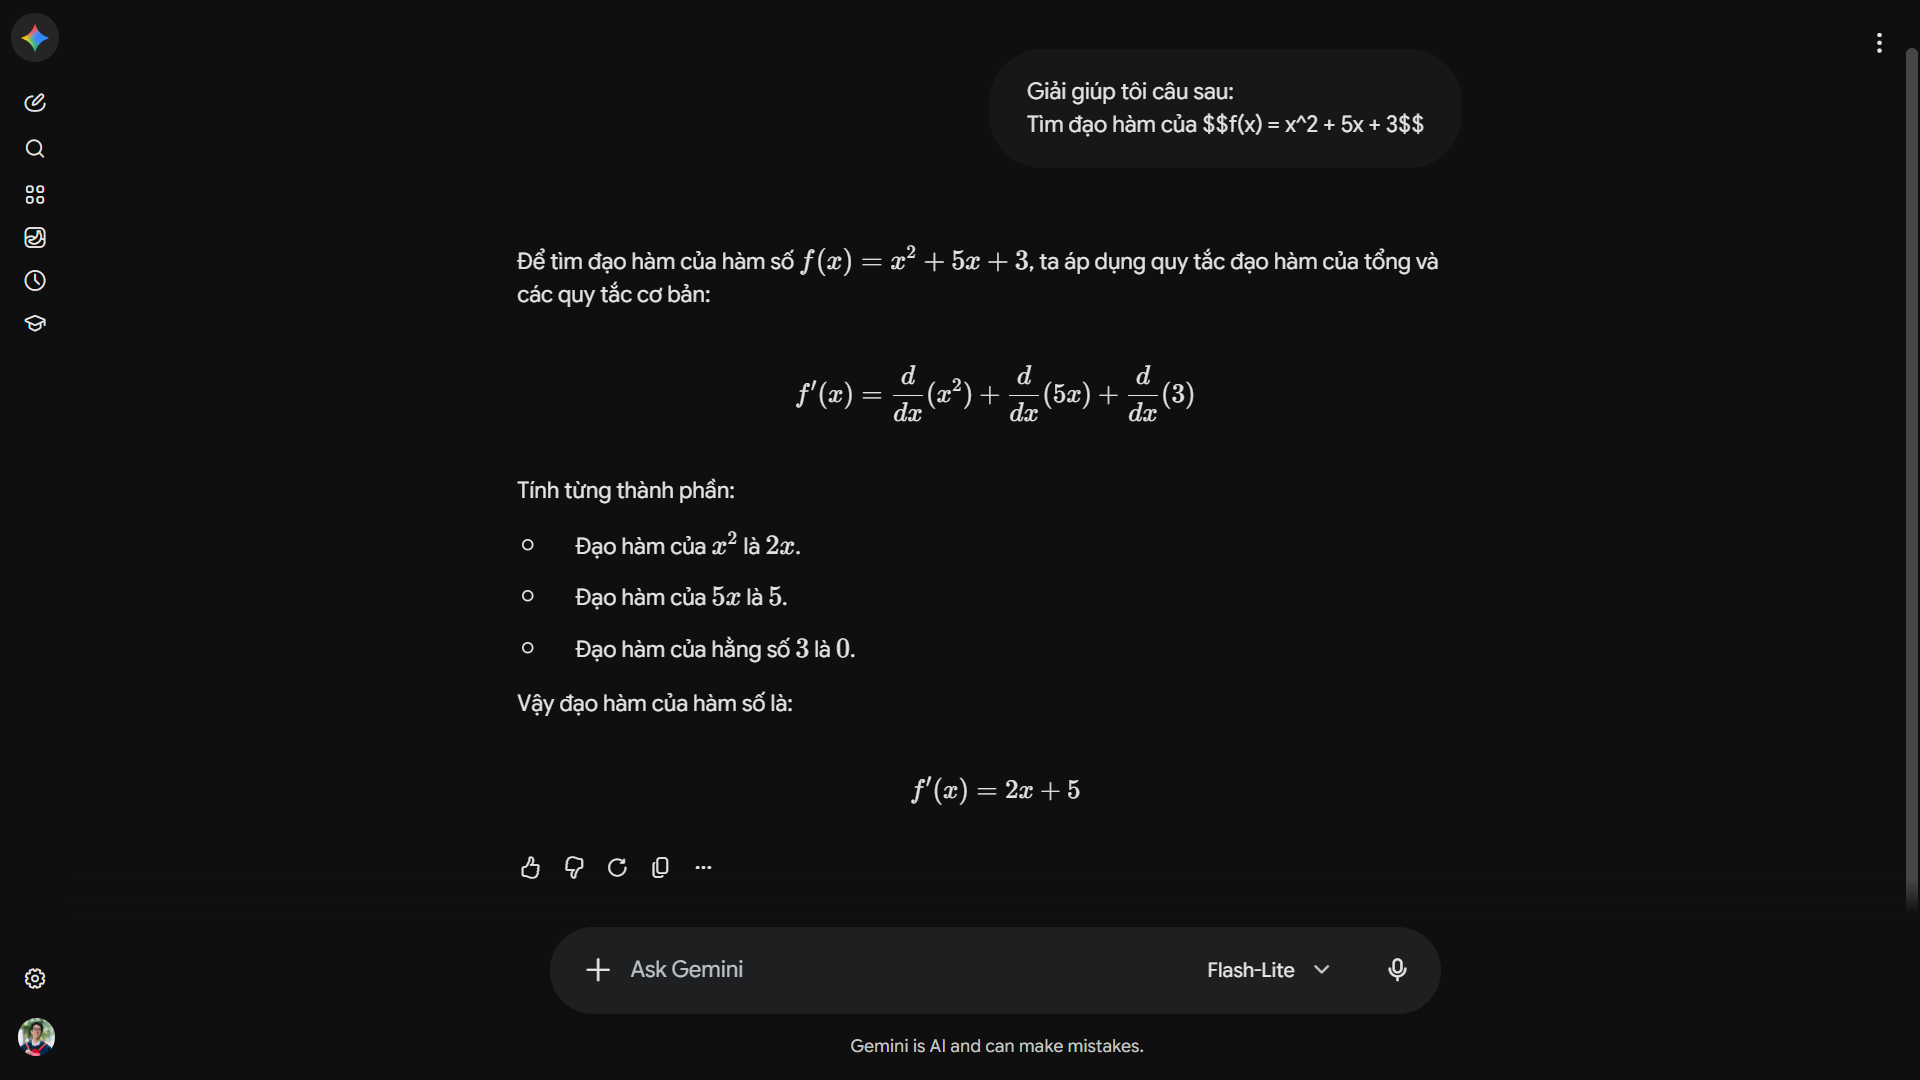
\includegraphics[width=0.72\textwidth]{anh1.png}
  \caption{Mô hình phân tích dễ hiểu, chi tiết cho người chưa biết có thể hiểu rõ từng bước làm}
  \label{fig:tot}
  \vspace{1mm}
  {\small\textit{(Đoạn chat thực tế:} \url{https://share.gemini.google/t2gbXH9W8Y2z}\textit{)}}
\end{figure}

\begin{figure}[H]
  \centering
  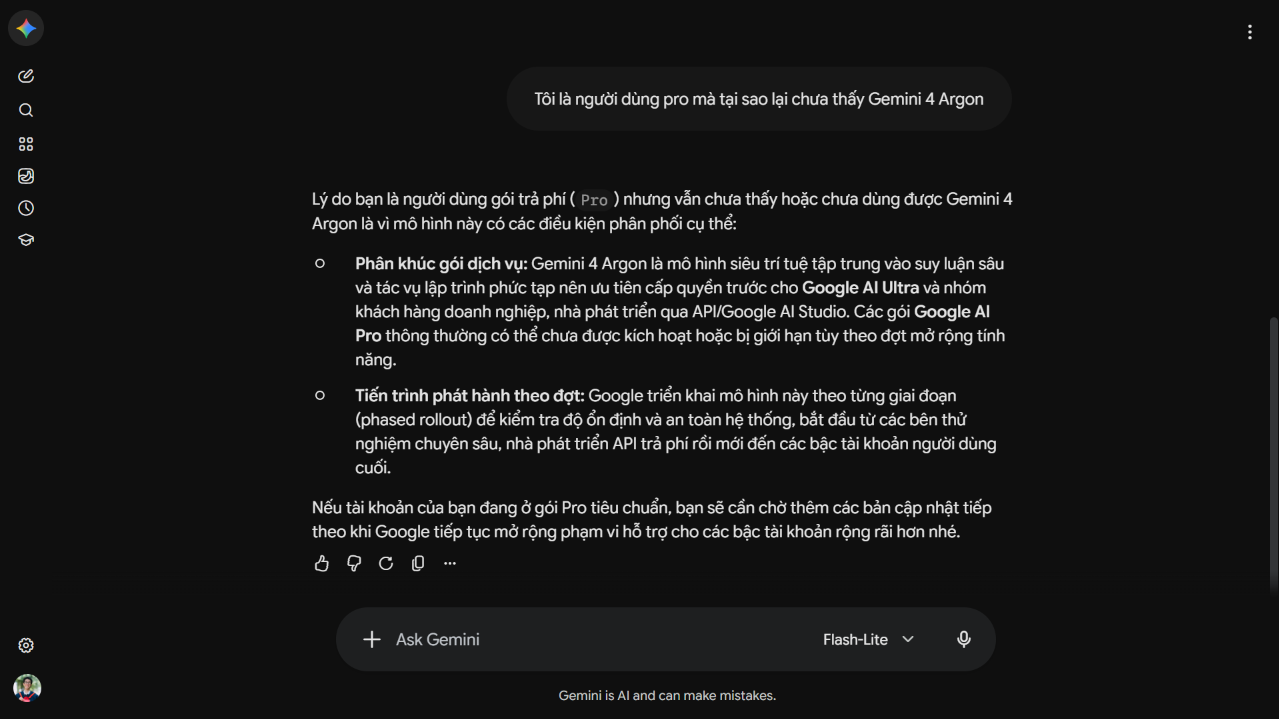
\includegraphics[width=0.72\textwidth]{anh2.png}
  \caption{Mô hình trả lời sai do tin theo thông tin không chính xác mà người dùng cung cấp}
  \label{fig:sai_sycophancy}
  \vspace{1mm}
  {\small\textit{(Đoạn chat thực tế:} \url{https://share.gemini.google/0lwOt5oaqwR5}\textit{)}}
\end{figure}

\begin{figure}[H]
  \centering
  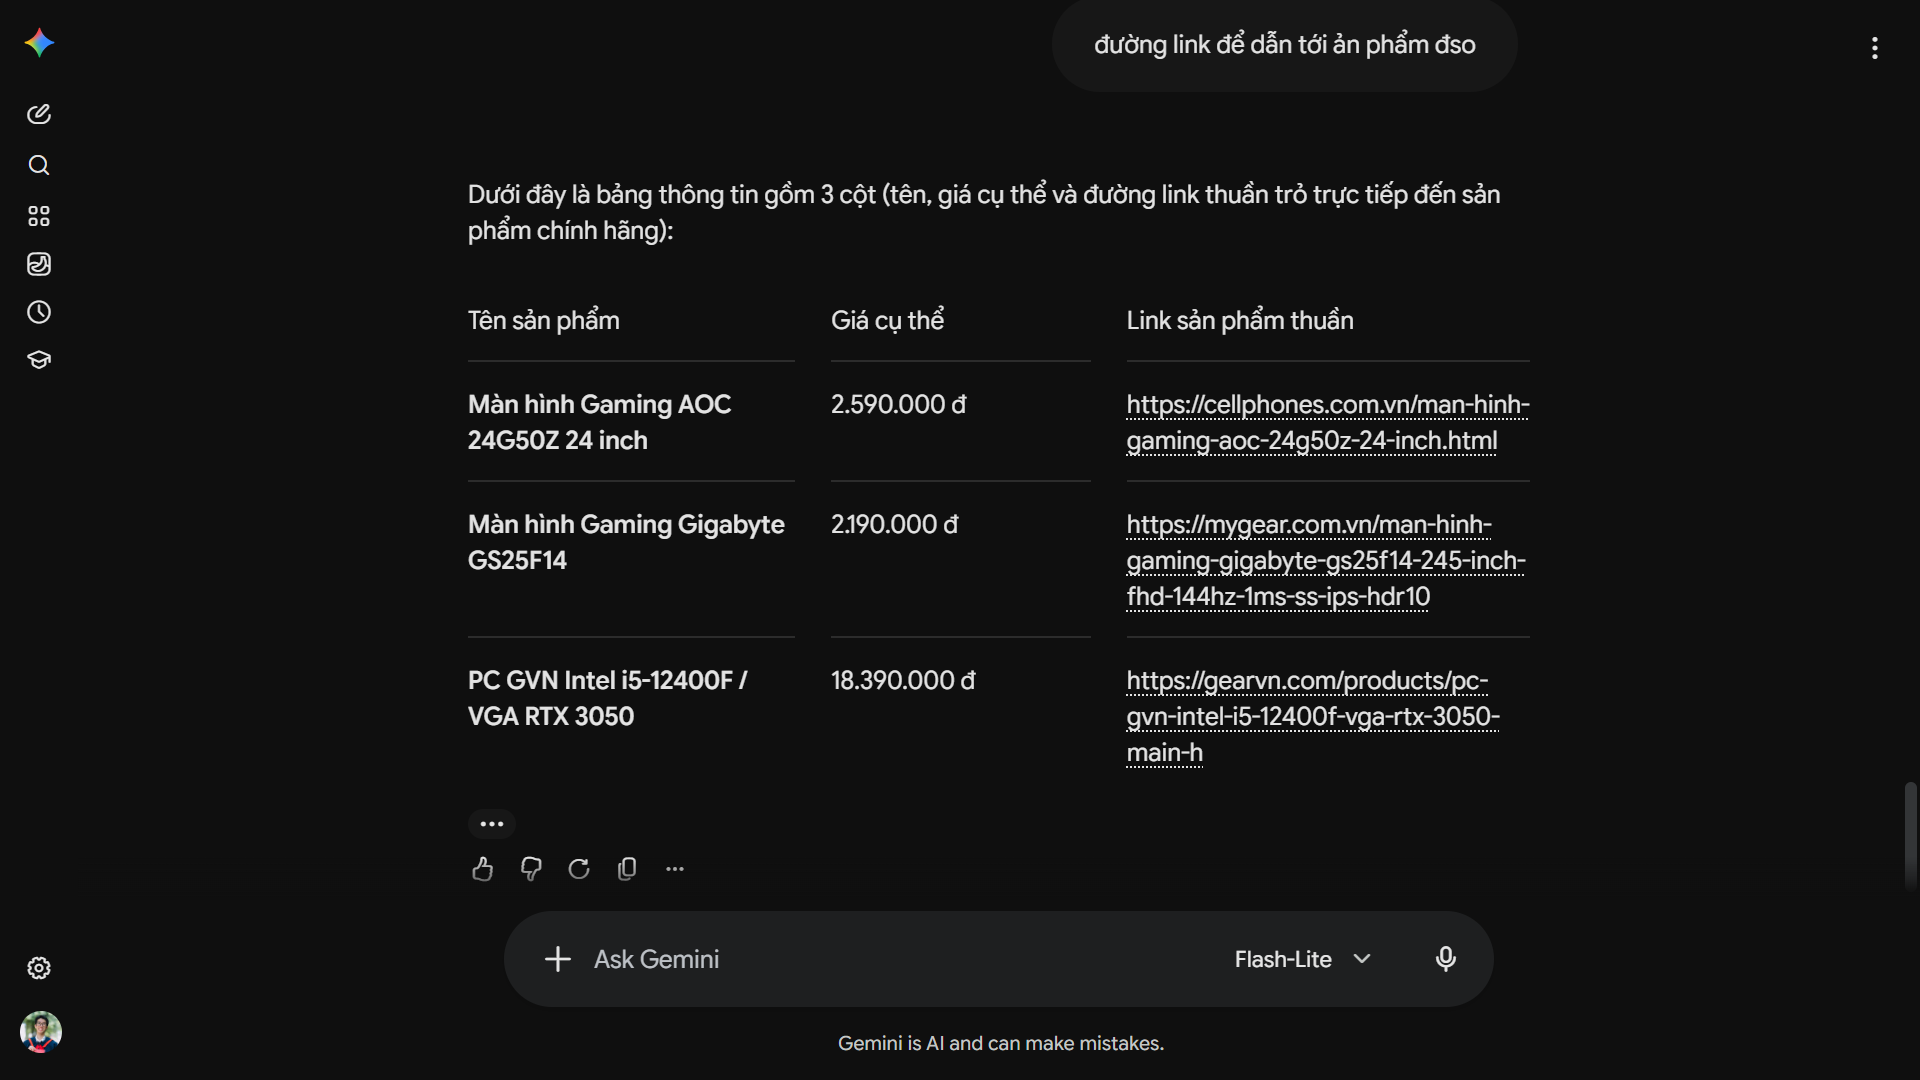
\includegraphics[width=0.72\textwidth]{anh3.png}
  \caption{Mô hình cung cấp các đường link không tồn tại trên thực tế}
  \label{fig:sai_link}
  \vspace{1mm}
  {\small\textit{(Đoạn chat thực tế:} \url{https://share.gemini.google/iy4SQsG7k5Gm}\textit{)}}
\end{figure}

\subsection{Nhận xét}
Qua các ví dụ trên, ta có thể thấy với các kiến thức rất cơ bản và phổ biến như là một định lý Toán học (Hình~\ref{fig:tot}) thì mô hình có thể làm rất tốt. Nhưng đối với các câu hỏi không phổ biến bằng hoặc quá mới, hoặc khi người dùng cố ý đưa ra một luận điểm sai (Hình~\ref{fig:sai_sycophancy}) thì có khả năng mô hình sẽ nghe theo và làm hài lòng người dùng thay vì phản bác%
\footnote{Bản chất lỗi này bắt nguồn từ giai đoạn căn chỉnh học tăng cường từ phản hồi con người (RLHF), khiến mô hình có xu hướng làm hài lòng con người theo cơ chế phần thưởng đã được học~\cite{casper2023open}.}.
Thêm vào đó, mô hình còn có thể tự tạo ra các đường link không tồn tại, hoàn toàn không sử dụng được (Hình~\ref{fig:sai_link}).

\section{Hạn chế và dùng có trách nhiệm}

\subsection{Hallucination (Ảo giác)}
\begin{itemize}
  \item Mô hình sinh ra các thông tin nghe rất học thuật và đáng tin cậy nhưng hoàn toàn sai sự thật (bịa tài liệu tham khảo, bịa công thức, suy diễn sai). Chi tiết ví dụ thể hiện rất rõ ở Hình~\ref{fig:sai_sycophancy} và Hình~\ref{fig:sai_link}.
  \item Phương pháp giảm thiểu: Sử dụng cơ chế RAG (Retrieval-Augmented Generation), yêu cầu trích dẫn nguồn, áp dụng quy trình kiểm chứng chéo (fact-checking) theo khảo sát của Tonmoy và cộng sự~\cite{tonmoy2024comprehensive}.
\end{itemize}

\subsection{Quyền riêng tư dữ liệu}
\begin{itemize}
  \item Dữ liệu người dùng nhập vào có thể được sử dụng để tái huấn luyện mô hình nếu không tắt cài đặt chia sẻ lịch sử.
  \item Nguy cơ rò rỉ mã nguồn nhạy cảm, thông tin cá nhân hoặc tài liệu nghiên cứu chưa công bố.
  \item \textbf{Ví dụ thực tế:} OpenAI tuyên bố một hệ thống AI nội bộ siêu việt giải được bài toán thiên niên kỷ nhưng vướng phải tranh cãi lớn khi bị tố cáo ăn cắp hướng đi nghiên cứu của nhà toán học qua việc sử dụng công cụ Codex~\cite{cafef-openai-dispute}.
  \item \textbf{Phương pháp giảm thiểu:} Cài đặt không chia sẻ dữ liệu (tắt lịch sử nếu có) và cẩn trọng khi đưa các dữ liệu quan trọng vào hỏi AI.
\end{itemize}

\subsection{Quy định dùng AI trong học tập}
Việc sử dụng AI trong môi trường giáo dục cần tuân thủ nghiêm ngặt các quy định về liêm chính học thuật~\cite{thuvienphapluat-ai-giaoduc}~\cite{ghimire2024generativeaieducationstudy}.

\subsubsection{Các quy định chính}
\begin{itemize}
  \item AI và công nghệ chỉ là công cụ hỗ trợ với vai trò người trợ giảng/cố vấn; người học phải chịu trách nhiệm 100\% về tính đúng đắn của sản phẩm cuối cùng.
  \item Việc dùng AI để gian lận là hành vi vi phạm liêm chính học thuật.
  \item Các ứng dụng công nghệ phải đảm bảo tính trung thực, khách quan, minh bạch, bảo mật dữ liệu và tôn trọng quyền sở hữu trí tuệ.
\end{itemize}

\subsubsection{Các hành vi vi phạm}
\begin{enumerate}
  \item Dùng AI để gian lận, sao chép, đạo văn hoặc làm sai lệch dữ liệu nghiên cứu.
  \item Nhờ người khác hoặc giao phó hoàn toàn cho AI thực hiện thay nhiệm vụ học tập, nghiên cứu.
  \item Không công bố hoặc công bố không đầy đủ việc sử dụng AI theo yêu cầu.
\end{enumerate}

\subsubsection{Trách nhiệm của cơ sở giáo dục}
Cơ sở giáo dục phải ban hành quy định nội bộ về liêm chính học thuật, xác định rõ chế tài, biện pháp phòng ngừa và trang bị hệ thống quản lý học tập hỗ trợ xác thực danh tính, lưu vết quá trình học tập nhằm ngăn chặn gian lận.

\section{Kết luận}

\subsection{Những kỹ năng khi sử dụng AI}
\begin{itemize}
  \item \textbf{Kỹ năng đặt câu hỏi (Prompting):} Biết cách diễn đạt yêu cầu rõ ràng, đầy đủ ngữ cảnh để AI hiểu đúng ý.
  \item \textbf{Kỹ năng tư duy phản biện:} Luôn hoài nghi và kiểm chứng lại câu trả lời của AI trước khi tin dùng.
\end{itemize}

\subsection{Định hướng sử dụng trong 4 năm đại học}
\begin{itemize}
  \item Xây dựng các công cụ tự động hóa bằng AI (Antigravity) để hỗ trợ việc học tập được hiệu quả hơn.
  \item Chỉ xem AI là bạn đồng hành, người trợ giảng hướng dẫn và gợi ý hướng đi, chứ không phải sử dụng AI để tạo sẵn đáp án rồi chép vào.
\end{itemize}

% =====================================================================
% [YC9] TÀI LIỆU THAM KHẢO — ít nhất 4 nguồn CÓ THẬT, khai báo trong refs.bib
% =====================================================================
\bibliographystyle{unsrt}
\bibliography{refs}

\newpage
% =====================================================================
% PHỤ LỤC BẮT BUỘC: NHẬT KÝ SỬ DỤNG AI
% =====================================================================
\appendix
\section{Nhật ký sử dụng AI}
Bảng~\ref{tab:nhatky} ghi nhận trung thực các phiên làm việc với AI theo đúng quy định AIAS 3 của môn học.

\begin{table}[H]
  \centering
  \caption{Nhật ký sử dụng AI chi tiết}
  \label{tab:nhatky}
  \begin{tabular}{p{3.6cm}p{5.2cm}p{5.8cm}}
    \toprule
    Prompt / Link hội thoại & AI giúp phần nào & Mình đã sửa lại gì \\
    \midrule
    \url{https://share.gemini.google/MXGnNn9FVFtC} & Soạn prompt nghiêm ngặt ban đầu, viết prompt để cho Agent không tự làm mọi thứ. & Củng cố thêm những yêu cầu như là không làm hộ, chỉ lập kế hoạch trước. \\
    \midrule
    Dự án Antigravity IDE (Khảo sát ngày 15/10/2026) & Hỗ trợ làm dàn ý mẫu (\texttt{draft.md}); chỉnh sửa nhẹ lỗi chính tả; hỗ trợ tìm nguồn bài báo; giải thích một số khái niệm như Transformer; chuyển nội dung sang định dạng \LaTeX{} chuẩn và đánh giá bài làm. & Tự triển khai bản nội dung chi tiết từ bản nháp (\texttt{content.md}); tự tra cứu và kiểm chứng dòng thời gian lịch sử mô hình; tự lấy BibTeX từ Google Scholar; tự sửa lại các đường link; sửa lại nhiều chi tiết khác còn chưa hợp lý. \\
    \midrule
    \url{https://share.gemini.google/XhbafID6cTah} & Cho biết thực tế có các loại token nào. & Bổ sung thông tin về các loại token đúng hơn so với bản \texttt{draft.md}. \\
    \midrule
    \url{https://share.gemini.google/t2gbXH9W8Y2z} & Ví dụ Hình~\ref{fig:tot}: giải thích định lý toán học. & Chụp hình câu trả lời thực tế để sử dụng trong bài. \\
    \midrule
    \url{https://share.gemini.google/0lwOt5oaqwR5} & Ví dụ Hình~\ref{fig:sai_sycophancy}: mô hình nghe theo luận điểm sai của người dùng. & Chụp hình câu trả lời thực tế để sử dụng trong bài. \\
    \midrule
    \url{https://share.gemini.google/iy4SQsG7k5Gm} & Ví dụ Hình~\ref{fig:sai_link}: mô hình sinh ra các đường link ảo giác. & Chụp hình câu trả lời thực tế để sử dụng trong bài. \\
    \bottomrule
  \end{tabular}
\end{table}

\section{Mã nguồn và tài nguyên thực nghiệm}
Toàn bộ mã nguồn \LaTeX{}, hình ảnh minh chứng và các tài liệu liên quan trong quá trình thực hiện bài tập được lưu trữ công khai tại kho mã nguồn GitHub: \url{https://github.com/<tai-khoan-github>/<ten-repo>}.

\end{document}
% [YC10] Trước khi nộp: tạo project mới trên Overleaf, upload file zip
% MSSV.zip, bấm Recompile — chạy được, không lỗi mới nộp.
